\documentclass[11pt,a4paper]{ivoa}
\usepackage[margin=4.25cm]{geometry} 
\input tthdefs
\setcounter{tocdepth}{2}

\title{Astronomical Measurements Model}

% see ivoatexDoc for what group names to use here
\ivoagroup{Data Model Working Group}

%\author[????URL????]{????Alfred Usher Thor????}
\author{Arnold Rots}
\author{Mark Cresitello-Dittmar}

\editor{Mark Cresitello-Dittmar}
\editor{Arnold Rots}

% \previousversion[????URL????]{????Funny Label????}
\previousversion{This is the first public release}
       

\begin{document}

\begin{abstract}
  In creating version 2 of ``\emph{Space-Time Coordinate Metadata for the Virtual Observatory}'' (STC) \citep{2007ivoa.spec.1030R} Data Model, it was decided to split the content into various component models which focus on particular aspects of the previous model scope.  
  
  This model covers the description of measured or determined astronomical data, and includes the following concepts:
  \begin{itemize}
  \item The association of the determined 'value' with corresponding errors.  In this model, the 'value' is given by the various Coordinate types of the Coordinates data model \citep{std:Coords}.
  \item A description of the Error model.
  \end{itemize}

\end{abstract}


\section*{Acknowledgments}
TBD: Get appropriate acknowledgment text

\section*{Conformance-related definitions}

The words ``MUST'', ``SHALL'', ``SHOULD'', ``MAY'', ``RECOMMENDED'', and
``OPTIONAL'' (in upper or lower case) used in this document are to be
interpreted as described in IETF standard RFC2119 \citep{std:RFC2119}.

The \emph{Virtual Observatory (VO)} is a
general term for a collection of federated resources that can be used
to conduct astronomical research, education, and outreach.
The \href{http://www.ivoa.net}{International
Virtual Observatory Alliance (IVOA)} is a global
collaboration of separately funded projects to develop standards and
infrastructure that enable VO applications.


\newgeometry{left=1.0in,right=1.0in,bottom=1.0in}
\section{Introduction}

\subsection{Motivation}
The collection and analysis of observed or derived data is the foundation of Astronomy.  
These data form the core of our most fundamental products:
\begin{itemize}
  \item Observational data - raw data in detector coordinates and instramental units.
  \item Derived data products - images and tables of derived data in physical units and coordinate spaces.
  \item Simulated data - data derived from simulation of physical entities and instrumentation.
  \item Catalogs - collections properties associated with various astronomical sources derived from multiple observations of that source.
\end{itemize}

Performing astronomical data analysis in the Virtual Observatory means to discover, evaluate, 
extract, combine and manipulate data which may have been obtained at different times, 
with different instruments, and different locations.  To confidently execute this workflow 
requires a complete and accurate description of the nature of the data and its associated errors.  

The ``\emph{Astronomical Coordinates and Coordinate Systems}'' (Coords) \citep{std:Coords} Data Model provides the description of the nature of the data values, the Coordinate space, reference frame, domain, etc.  Here, we utilize that information to build a model for observed or derived data which adds elements quantifying the accuracy of the data.

\subsection{Context and Scope}

This document results from updating the ``\emph{Space-Time Coordinate Metadata for the Virtual Observatory}'' (STC) \citep{2007ivoa.spec.1030R} model for use in VO-DML compliant models.  That model provides metadata for describing Space-Time related, and other Coordinates including associated errors.  These metadata are to be used for specifying coordinate-related information for datasets, catalogs, and queries.  In this work, our primary focus is to support the use cases described below, while keeping the broader scope in mind to inform design decisions for future expansion.

The update and revision of the STC model has sub-divided the content into component models, each covering a portion of the scope of the parent model.  This allows for better description of the relations between the various components, allows for independent development of the component models, and creates smaller, more digestible content for users.

In the astronomical community, the terms ``quantity'', ``coordinate'', and ``measurement'' are used interchangably, but not always with the same meaning.  The ``coordinate'' of a star is typically a measured location, while the ``coordinate'' of the center of a circular region is not.  We provide here a short glossary of these terms in the IVOA data model context.
\begin{itemize}
  \item Quantity: [ivoa model]  A number with a unit.
  \item Coordinate: [coords model]  An absolute location within a coordinate space.  Comprised of a 'value' (often a Quantity), associated with an axis in a coordinate space, and a coordinate frame providing additional metadata about the orientation and origin of the coordinate space.  In other words, a location in a domain space.
  \item Measurement: [meas model]  For 'measured', or 'determined' data.  Combines a Coordinate (ie: the determined value) with corresponding Error(s).  For the majority of cases dealing with astronomical data, this is what we are referring to.
\end{itemize}

This document describes the Measurement model which provides descriptions for:
\begin{itemize}
  \item The observed or derived data 'value'.
  \item The error(s) associated with that 'value'.
\end{itemize}

\section{Use Cases and Requirements}
\label{sect:ucreq}

\subsection{Use Cases}
\label{sect:usecases}

\subsubsection{Cube model support}
\label{uc:Cube-model-support}
  The primary use case for this work is in support of the CubesDM. \\
  The CubesDM is a N-Dimensional model for pixelated images and sparse cube data. 
 
  The following is a brief outline of the most relevant features pertaining to the
  development of the Measurement, Coordinates, and Transform component models.  Many 
  of these features are handled by the Coordinates or Transform models, but are 
  relevant to the full description of Measurement model elements.

  \begin{itemize}
    \item General
    \begin{itemize}
       \item knowledge of the physical domain spaces provided at a high level
       \item definition of the domain space includes the following criteria
       \begin{itemize}
          \item dimensionality (typically 1,2 or 3 for physical domain), pixel domain may be of any dimension
          \item axis configuration (for spatial domain which has >1D).  The most common configurations for astronomical data are Cartesian and Spherical, but others may be used as well.
          \item domain range along each axis, typically +/- Inf, but may be limited due to physical constraints (e.g. physical size of a detector, sensitivity limitiations, etc)
          \item association with additional metadata further describing the nature of the domain space ( Frame ).  This is especially true for the Spatial and Temporal domains, but may apply to others as well.  Examples include:
          \begin{itemize}
             \item reference position (location of origin)
             \item reference frame (orientation of the domain space)
             \item planetary ephemeris
             \item equinox
          \end{itemize}
       \end{itemize}
    \end{itemize}
    \item Pixelated Image Cube
    \begin{itemize}
       \item complete specification of pixel coordinate domain; number of axes, number of pixels per axis
       \item image axes
       \begin{itemize}
          \item in pixel domain, are a binned coordinate space with integerized values (pixel indexes) 
          \item mapped to various 'physical' coordinate spaces via transform operations 
          \item mappings may define a progressive migration in coordinate space (e.g. pixel - ccd - detector - sky - wcs ) 
          \item pixel axis mappings are typically to a continuous domain, but may also be to a discrete domain such as Polarization state.
       \end{itemize}
       \item image cubes may have any number of dimensions, but are typically separable into co-dependent axes of 1, 2, or 3 dimensions.
       \begin{itemize}
          \item spatial domain typically 2-3 dimensions
          \item other domains (time, spectral, polarization), are typically 1 dimensional
       \end{itemize}
       \item image data value is typically given in a physical domain, but may itself be mapped to other domains
    \end{itemize}
    \item Sparse Cube
    \begin{itemize}
       \item data axes cover a wide array of physical domains including, but not limited to Spatial, Temporal, Spectral, Polarization,
       \item individual domains may be represented multiple times in different frames ( ccd, detector, sky;  pha, energy )
       \item data values may have associated errors
       \begin{itemize}
          \item typical error forms include: symmetric( +/- a ), asymmetric( +a:-b ), interval ( a:b ), matrix, elliptical
          \item can become quite complex: probability distributions, error maps, etc.
          \item quality indicators:
          \begin{itemize}
             \item global status, typically numeric
             \item bit array, where each bit is associated with a particular quality state 
          \end{itemize}
          \item associated errors may be separable or correlated among multiple data axes
        \end{itemize}
        \item data axes may be virtual, defined as a mapping from other data axes (same description as above)
    \end{itemize}
    \item Physical Data (Observables)
    \begin{itemize}
       \item focus on the following domains which are frequently included in astronomical data cubes: Spatial, Spectral, Temporal, Polarization
       \item Spatial
       \begin{itemize}
          \item Cartesian space:  chip, detector, sky
          \item Spherical space: Equatorial, Ecliptic, Galactic, LongLat
       \end{itemize}
       \item Time
       \begin{itemize}
          \item 1-Dimensional: JD, MJD, ISOTime, TimeOffset
       \end{itemize}
       \item Polarization
       \begin{itemize}
          \item Discrete space: Polarization states (Stokes, Linear, Circular, Vector )
       \end{itemize}
       \item Spectral
       \begin{itemize}
          \item 1-Dimensional: energy, frequency, wavelength
       \end{itemize}
    \end{itemize}
  \end{itemize}

\subsection{Requirements}
\label{sect:reqs}

 Examination and implementation of the above cases leads to a set of requirements distributed through the various STC component models.  Here we 
itemize those relevant to this model specifically.

\subsubsection{General}
Requirements pertaining to the overall criteria that the model must satisfy.
  \begin{itemize}
    \item [\textbf{[vodml.001]:}] The model shall be vo-dml compliant
    \item [\textbf{[vodml.002]:}] shall re-use, or refer to, dependent models for objects and concepts already defined in other models
    \item [\textbf{[vodml.003]:}] shall produce a validated vo-dml XML description
    \item [\textbf{[vodml.004]:}] shall produce documentation in vo-dml HTML format
    \item [\textbf{[vodml.005]:}] shall produce documentation in standard PDF format
  \end{itemize}

\subsubsection{Application/Usage}
Requirements pertaining to the user experience.  Note, as a data model, users will not typically interact directly with the model,
  \begin{itemize}
    \item [\textbf{[user.001]:}] Users should be able to identify and use basic content with minimal specialized information. 
      In other words, a generic utility should be able to find and use core elements without knowing a lot about the various extensions and uses of those elements.
    \item [\textbf{[user.002]:}] When applicable, the model should support usability by simplifying common scenarios. i.e. common things simple, complex things possible
    \item [\textbf{[user.003]:}] The model shall be easily extended to accommodate cases and applications not yet considered.
  \end{itemize}

\subsubsection{Content}
Requirements pertaining to the elements to be defined by the model.
\begin{itemize}
  \item Domains
  \begin{itemize}
    \item [\textbf{[dom.001]:}] Shall accommodate the description of data in any observable domain
    \item [\textbf{[dom.002]:}] Shall provide enhanced/specialized description for data pertaining to
    \begin{itemize}
      \item [\textbf{[dom.002.1]:}] Pixel domain: binned, integerized, n-dimensional domain
      \item [\textbf{[dom.002.2]:}] Spatial domain: continuous domain, typically in 2-3 dimensional cartesian or spherical spaces
      \item [\textbf{[dom.002.3]:}] Time domain: continuous 1D domain, typically provided in JD, MJD, ISO, or as an Offset from a zero point
      \item [\textbf{[dom.002.4]:}] Polarization domain: discrete 1D domain of polarization states. 
    \end{itemize}
  \end{itemize}

  \item Measurements
  \begin{itemize}
    \item [\textbf{[meas.001]:}] Shall relate a coordinate value with associated errors
    \item [\textbf{[meas.002]:}] Shall support multiple error associations per value to describe errors from different sources
    \item [\textbf{[meas.003]:}] A value must not be associated with more than one each of statistical and systematic errors
    \item [\textbf{[meas.004]:}] Errors may be correlated between component values ( ie: may apply to coordinate set as a whole )
    \item [\textbf{[meas.005]:}] Values associated with different domains may have correlated errors (ie: components of coordinate tuple may refer to different domains, and have non-separable errors)
    \item [\textbf{[meas.006]:}] Shall support the most common error forms, including, but not limited to: Symmetrical, Asymmetrical, Interval, Elliptical \\ with assumed Gaussian distribution at a 1-sigma confidence level.
    \item [\textbf{[meas.007]:}] Shall provide specialized objects related to measurements in the priority domains ( Spatial, Spectral, Temporal, Polarization ); leveraging [user.0002] where possible
    \item [\textbf{[meas.008]:}] Shall allow for the representation data outside the priority domains 
  \end{itemize}
\end{itemize}


\pagebreak
\subsection{Role within the VO Architecture}

\begin{figure}[h]
\centering

% As of ivoatex 1.2, the architecture diagram is generated by ivoatex in
% SVG; copy ivoatex/archdiag-full.xml to archdiag.xml and throw out
% all lines not relevant to your standard.
% Notes don't generally need this.  If you don't copy archdiag.xml,
% you must remove archdiag.svg from FIGURES in the Makefile.

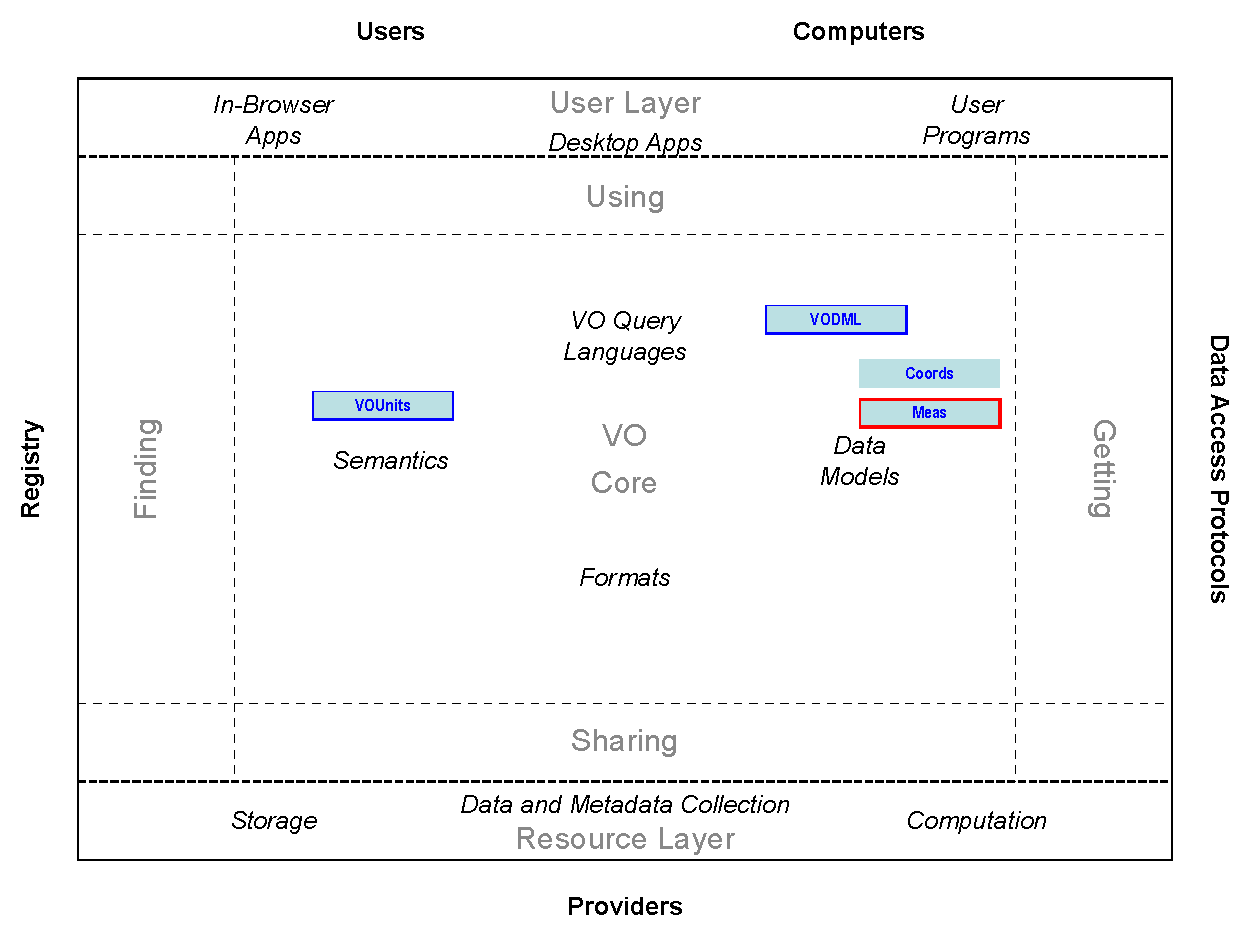
\includegraphics[width=0.9\textwidth]{role_diagram.pdf}
\caption{Architecture diagram for this document}
\label{fig:archdiag}
\end{figure}

Fig.~\ref{fig:archdiag} shows the role this document plays within the
IVOA architecture \citep{2010ivoa.rept.1123A}.

% Main Body of the document, extracted from vo-dml/xml using vo-dml2ivoatex
% with some post-processing.

% -------------------------------------------
% Items to substitute into the ivoatex document template.
%
%\ivoagroup{Data Model Working Group}

%\title{Astronomical Measurements Model}


%\author{Arnold Rots}
    
%\author{Mark Cresitello-Dittmar}
    
%\author{Omar Laurino}
    
%\previousversion{0.x}
      
% -------------------------------------------

\pagebreak
\section{Model: meas }
  
  % INSERT FIGURE HERE
  \begin{figure}[h]
  \begin{center}
    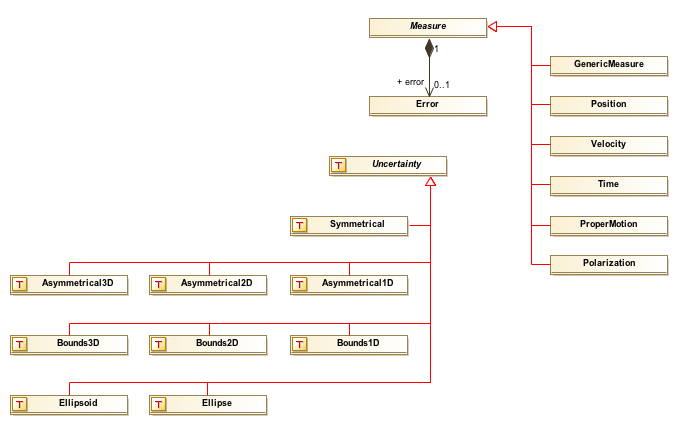
\includegraphics[width=5.75in]{diagrams/Overview.png}
    \caption{Overview of Measurement model elements}\label{fig:overview}
  \end{center}
  \end{figure}

  This model defines objects and datatypes which represent 'measured' or 'determined' data. It associates a Coordinate (ie: the determined value with associated physical context) with corresponding Error(s). As such, this model is at least the foundation for representing the vast majority of the Astronomical data found in catalogs and data products. 

We define here, several specialized classes which cover the most basic and common types, such as Position and Time. We also provide a generic model which can accommodate virtually any data, but may require a bit more effort to fully describe the coordinate metadata. Additional specializations, e.g. Flux, Magnitude, Luminosity, Pressure, Temperature, etc. may be added to this model, or in other models focusing on particular domains or use cases. 

We include a fairly simple Error model, describing errors as a 'shape' of uncertainty, and define a small set of commonly occuring forms (e.g. Symmetrical, Bounds, Ellipsoid).

\pagebreak
\section{Measure}

  % INSERT FIGURE HERE
  \begin{figure}[h]
  \begin{center}
    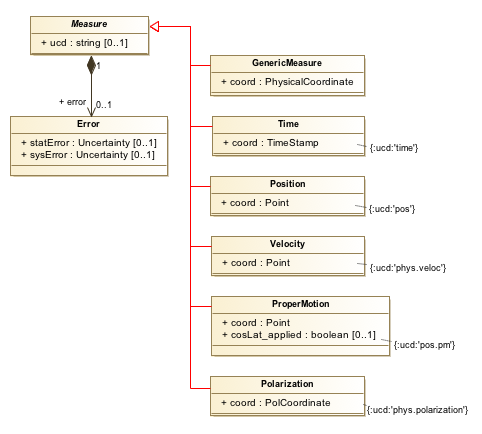
\includegraphics[width=3.5in]{diagrams/Measure.png}
    \caption{Measure elements}\label{fig:measure}
  \end{center}
  \end{figure}

  \subsection{Measure (Abstract)}
  \label{sect:Measure}
    Abstract base of Measure classes, associates a 'determined value' (Coordinate) with corresponding errors.

    The breadth of astronomical data makes it impractical to define specialized classes for each property which may be measured or determined. In this model, we take a two-pronged approach for identifying the nature of any given Measure. First, we allow the use of a Unified Content Descriptor (UCD) to convey this information. Second, we define specialized classes for properties which either have additional metadata associated with them, have complex coordinate spaces, and/or have special significance in other models. For these specialized classes, the ucd is constrained to a fixed value.

    We associate the Error(s) with the full Measure, rather than the individual values, in order to support both correlated and uncorrelated errors. In many cases with multi-dimensional data, the associated errors are correlated and must be considered with the value set as a whole. One consequence of this approach is that there is a looser association between the Error dimensions and the corresponding value dimension. We require that the Error content MUST be compatible with the value dimension and nature (e.g. dimension, domain, units, etc).

    \subsubsection{Measure.ucd}
      \textbf{vodml-id: Measure.ucd} \newline
      \textbf{type: \hyperref[sect:ivoa]{ivoa:string}} \newline
      \textbf{multiplicity: 0..1} \newline 
      The Unified Content Descriptor (UCD) defines a controlled vocabulary for describing astronomical quantities. Other than in the specialized types, we only constrain ucd value to being valid according to the vocabulary syntax. However, the intent is to use only enough of the vocabulary to convey the nature of the measured value, and avoid usage of terms which may overlap with modeled concepts associated with the value. For example, borrowing from examples in the UCD document: for a magnitude measured in the J band, the ucd "phot.mag" is preferred over "phot.mag;em.IR.J" which conveys information about an associated filter, or "phot.mag;em.IR.J;meta.modelled" which includes ancillary qualifiers.

    \subsubsection{Measure.error}
      \textbf{vodml-id: Measure.error} \newline
      \textbf{type: \hyperref[sect:Error]{meas:Error}} \newline
      \textbf{multiplicity: 0..1} \newline 
      Measurement error.

  \subsection{Error}
  \label{sect:Error}
    The Error class uses the Uncertainty types to describe measurement errors from various sources.

    \subsubsection{Error.statError}
      \textbf{vodml-id: Error.statError} \newline
      \textbf{type: \hyperref[sect:Uncertainty]{meas:Uncertainty}} \newline
      \textbf{multiplicity: 0..1} \newline 
      Statistical error. The Uncertainty type MUST be dimensionally compatible with the associated Measure value.

    \subsubsection{Error.sysError}
      \textbf{vodml-id: Error.sysError} \newline
      \textbf{type: \hyperref[sect:Uncertainty]{meas:Uncertainty}} \newline
      \textbf{multiplicity: 0..1} \newline 
      Systematic error. The Uncertainty type MUST be dimensionally compatible with the associated Measure value.


  \subsection{GenericMeasure}
  \label{sect:GenericMeasure}
    The most generic Measure class. This class may be used to represent data not covered by the specialized cases.

    \subsubsection{GenericMeasure.coord}
      \textbf{vodml-id: GenericMeasure.coord} \newline
      \textbf{type: coords:PhysicalCoordinate} \newline
      \textbf{multiplicity: 1} \newline 
      The measured coordinate value.

  \subsection{Time}
  \label{sect:Time}
    Provides a complete description of a measured Temporal instant.

    \noindent \textbf{constraint} \newline
    \indent    \textbf{detail: Time.ucd:'time' }\newline

    \subsubsection{Time.coord}
      \textbf{vodml-id: Time.coord} \newline
      \textbf{type: coords:TimeStamp} \newline
      \textbf{multiplicity: 1} \newline 
      The measured time value. May be provided in any of the TimeStamp subtypes.


  \subsection{Position}
  \label{sect:Position}
    Provides a complete description of a measured positional instant.

    \noindent \textbf{constraint} \newline
    \indent    \textbf{detail: Position.ucd:'pos' }\newline

    \subsubsection{Position.coord}
      \textbf{vodml-id: Position.coord} \newline
      \textbf{type: coords:Point} \newline
      \textbf{multiplicity: 1} \newline 
      The measured Position value. The Point coordinate supports 1,2, and 3-dimensional cases. Details of the coordinate system (space and frame), are associated with the Point.


  \subsection{Velocity}
  \label{sect:Velocity}
    Provides a comple description of a measured Velocity instant.

    \noindent \textbf{constraint} \newline
    \indent    \textbf{detail: Velocity.ucd:'phys.veloc' }\newline

    \subsubsection{Velocity.coord}
      \textbf{vodml-id: Velocity.coord} \newline
      \textbf{type: coords:Point} \newline
      \textbf{multiplicity: 1} \newline 
      The measured Velocity value. The Point coordinate supports 1,2, and 3-dimensional cases. Details of the coordinate system (space and frame), are associated with the Point.


  \subsection{ProperMotion}
  \label{sect:ProperMotion}
    Proper motion represented as the velocity in Longitude and Latitude directions of a spherical coordinate space. The associated SpaceFrame provides the details regarding the nature of the coordinate space (eg: Equatorial, Galactic, etc).

    \noindent \textbf{constraint} \newline
    \indent    \textbf{detail: ProperMotion.ucd:'pos.pm' }\newline

    \subsubsection{ProperMotion.coord}
      \textbf{vodml-id: ProperMotion.coord} \newline
      \textbf{type: coords:Point} \newline
      \textbf{multiplicity: 1} \newline 
      Velocity in angular distance per unit time. We use the Point type for the proper motion value to be consistent with the Position and Velocity types, allowing representation in different coordinate spaces (eg: Polar).

    \subsubsection{ProperMotion.cosLat\_applied}
      \textbf{vodml-id: ProperMotion.cosLat\_applied} \newline
      \textbf{type: \hyperref[sect:ivoa]{ivoa:boolean}} \newline
      \textbf{multiplicity: 0..1} \newline 
      It is common, though not universal, practice to quote longitudinal proper motion pre-multiplied by cos(latitude) so that the magnitude of the quantity is not affected by its longitudinal position. We do not constrain the value to one form or the other in this model. Instead, this flag enables providers to convey whether or not the factor has been applied.

  \subsection{Polarization}
  \label{sect:Polarization}
    Provides a complete description of a determined polarization state. Since the polarization coordinate is an enumerated type, there can be no associated numerical error sources.

    \noindent \textbf{constraint} \newline
    \indent    \textbf{detail: Polarization.error:Error[0] }\newline

    \noindent \textbf{constraint} \newline
    \indent    \textbf{detail: Polarization.ucd:'phys.polarization' }\newline

    \subsubsection{Polarization.coord}
      \textbf{vodml-id: Polarization.coord} \newline
      \textbf{type: coords:PolCoordinate} \newline
      \textbf{multiplicity: 1} \newline 
      Determined polarization state. May be provided by any of the PolCoordValue subtypes.

\pagebreak
\section{Uncertainty}

  % INSERT FIGURE HERE
  \begin{figure}[h]
  \begin{center}
    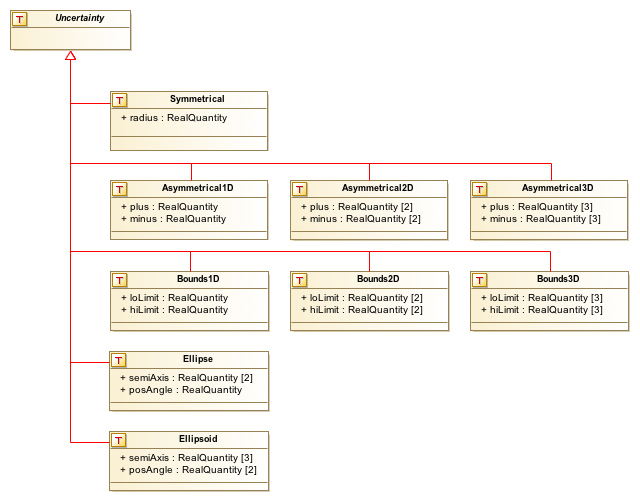
\includegraphics[width=5in]{diagrams/Uncertainty.png}
    \caption{Uncertainty elements}\label{fig:uncertainty}
  \end{center}
  \end{figure}

  \subsection{Uncertainty (Abstract)}
  \label{sect:Uncertainty}
    Abstract head of uncertainty types. These classes define the shape of the uncertainty, and are designed to be reusable in different contexts. Uncertainties are designed to be associated with a Coordinate or other object which provides the 'center' or reference location about which the uncertainty resides. 

In this model, we use them in the context of defining measurement errors, but they are also compatible for use in defining resolutions which are to be modeled at a later date. This initial version of the model forms a fundamental basis which can then be expanded to include more complex and varied use cases as they present themselves. The current model assumes Gaussian distributions with shapes defined at the 68\% confidence level.

  \subsection{Symmetrical}
  \label{sect:Symmetrical}
    Symmetrical uncertainty, constant in all dimensions and directions from the associated Coordinate. ie: PlusMinus in 1D, circular in 2D, spherical in 3D.

    \subsubsection{Symmetrical.radius}
      \textbf{vodml-id: Symmetrical.radius} \newline
      \textbf{type: \hyperref[sect:ivoa]{ivoa:RealQuantity}} \newline
      \textbf{multiplicity: 1} \newline 
      The uncertainty extent, constant in all dimensions and directions.

  \subsection{Asymmetrical1D}
  \label{sect:Asymmetrical1D}
    Uncertainty with different extent in the positive and negative directions from the associated Coordinate.

    \subsubsection{Asymmetrical1D.plus}
      \textbf{vodml-id: Asymmetrical1D.plus} \newline
      \textbf{type: \hyperref[sect:ivoa]{ivoa:RealQuantity}} \newline
      \textbf{multiplicity: 1} \newline 
      Extent in the positive axis direction.

    \subsubsection{Asymmetrical1D.minus}
      \textbf{vodml-id: Asymmetrical1D.minus} \newline
      \textbf{type: \hyperref[sect:ivoa]{ivoa:RealQuantity}} \newline
      \textbf{multiplicity: 1} \newline 
      Extent in the negative axis direction.

  \subsection{Asymmetrical2D}
  \label{sect:Asymmetrical2D}
    2D Uncertainty with different extent in the positive and negative axis directions from the associated Coordinate. i.e.: an offset rectangle.

    \subsubsection{Asymmetrical2D.plus}
      \textbf{vodml-id: Asymmetrical2D.plus} \newline
      \textbf{type: \hyperref[sect:ivoa]{ivoa:RealQuantity}} \newline
      \textbf{multiplicity: 2} \newline 
      Extent in each positive axis direction.

    \subsubsection{Asymmetrical2D.minus}
      \textbf{vodml-id: Asymmetrical2D.minus} \newline
      \textbf{type: \hyperref[sect:ivoa]{ivoa:RealQuantity}} \newline
      \textbf{multiplicity: 2} \newline 
      Extent in each negative axis direction.

  \subsection{Asymmetrical3D}
  \label{sect:Asymmetrical3D}
    3D Uncertainty with different extent in the positive and negative axis directions from the associated Coordinate. i.e.: an offset box.

    \subsubsection{Asymmetrical3D.plus}
      \textbf{vodml-id: Asymmetrical3D.plus} \newline
      \textbf{type: \hyperref[sect:ivoa]{ivoa:RealQuantity}} \newline
      \textbf{multiplicity: 3} \newline 
      Extent in each positive axis direction.

    \subsubsection{Asymmetrical3D.minus}
      \textbf{vodml-id: Asymmetrical3D.minus} \newline
      \textbf{type: \hyperref[sect:ivoa]{ivoa:RealQuantity}} \newline
      \textbf{multiplicity: 3} \newline 
      Extent in each negative axis direction.

  \subsection{Bounds1D}
  \label{sect:Bounds1D}
    Provide the edges of the uncertainty space. Rather than being relative to the associated Coordinate, these represent a range within that Coordinate space.

    \subsubsection{Bounds1D.loLimit}
      \textbf{vodml-id: Bounds1D.loLimit} \newline
      \textbf{type: \hyperref[sect:ivoa]{ivoa:RealQuantity}} \newline
      \textbf{multiplicity: 1} \newline 
      Lower limit of the uncertainty range.

    \subsubsection{Bounds1D.hiLimit}
      \textbf{vodml-id: Bounds1D.hiLimit} \newline
      \textbf{type: \hyperref[sect:ivoa]{ivoa:RealQuantity}} \newline
      \textbf{multiplicity: 1} \newline 
      Upper limit of the uncertainty range.

  \subsection{Bounds2D}
  \label{sect:Bounds2D}
    Provide the edges of a 2D uncertainty space. Rather than being relative to the associated Coordinate, these represent ranges along each axis of that Coordinate space.

    \subsubsection{Bounds2D.loLimit}
      \textbf{vodml-id: Bounds2D.loLimit} \newline
      \textbf{type: \hyperref[sect:ivoa]{ivoa:RealQuantity}} \newline
      \textbf{multiplicity: 2} \newline 
      Lower edges of the uncertainty rectangle.

    \subsubsection{Bounds2D.hiLimit}
      \textbf{vodml-id: Bounds2D.hiLimit} \newline
      \textbf{type: \hyperref[sect:ivoa]{ivoa:RealQuantity}} \newline
      \textbf{multiplicity: 2} \newline 
      Upper edges of the uncertainty rectangle.

  \subsection{Bounds3D}
  \label{sect:Bounds3D}
    Provide the edges of a 3D uncertainty space. Rather than being relative to the associated Coordinate, these represent ranges along each axis of that Coordinate space.

    \subsubsection{Bounds3D.loLimit}
      \textbf{vodml-id: Bounds3D.loLimit} \newline
      \textbf{type: \hyperref[sect:ivoa]{ivoa:RealQuantity}} \newline
      \textbf{multiplicity: 3} \newline 
      Lower edges of the uncertainty box.

    \subsubsection{Bounds3D.hiLimit}
      \textbf{vodml-id: Bounds3D.hiLimit} \newline
      \textbf{type: \hyperref[sect:ivoa]{ivoa:RealQuantity}} \newline
      \textbf{multiplicity: 3} \newline 
      Upper edges of the uncertainty box.

  \subsection{Ellipse}
  \label{sect:Ellipse}
    Elliptical uncertainty shape.

    \subsubsection{Ellipse.semiAxis}
      \textbf{vodml-id: Ellipse.semiAxis} \newline
      \textbf{type: \hyperref[sect:ivoa]{ivoa:RealQuantity}} \newline
      \textbf{multiplicity: 2} \newline 
      Extent of the semi-major and semi-minor axes, provided in the order of the associated Coordinate axes.

    \subsubsection{Ellipse.posAngle}
      \textbf{vodml-id: Ellipse.posAngle} \newline
      \textbf{type: \hyperref[sect:ivoa]{ivoa:RealQuantity}} \newline
      \textbf{multiplicity: 1} \newline 
      Position angle, counter-clockwise from the positive direction of the first axis of the associated Coordinate. When used in the spatial domain, the expectation is that the 'first axis' corresponds to the 'North Celestial Pole', and the second to 'East', thereby conforming to the IAU definition of the position angle direction being 'East of North'.

  \subsection{Ellipsoid}
  \label{sect:Ellipsoid}
    Ellipsoidal uncertainty shape.

    \subsubsection{Ellipsoid.semiAxis}
      \textbf{vodml-id: Ellipsoid.semiAxis} \newline
      \textbf{type: \hyperref[sect:ivoa]{ivoa:RealQuantity}} \newline
      \textbf{multiplicity: 3} \newline 
      Extent of the semi axes, provided in the order of the associated Coordinate axes.

    \subsubsection{Ellipsoid.posAngle}
      \textbf{vodml-id: Ellipsoid.posAngle} \newline
      \textbf{type: \hyperref[sect:ivoa]{ivoa:RealQuantity}} \newline
      \textbf{multiplicity: 2} \newline 
      Position angles
      \begin{enumerate}
      \item counter-clockwise from the positive direction of the first axis toward the second axis
      \item angle 'above' the plane of the first two axes of the associated Coordinate
      \end{enumerate}
      When used in the spatial domain, the expectation is that the 'first axis' corresponds to the 'North Celestial Pole', and the second to 'East', thereby conforming to the IAU definition of the position angle direction being 'East of North'.



\pagebreak
\appendix
\section{Changes from Previous Versions}

% No previous versions yet.  

% these would be subsections "Changes from v. WD-..."
% Use itemize environments.
\subsection{Changes from PR-2020-04-13}
\begin{itemize} 
  \item update citation codes per ivoatex changes.
  \item Section 4.1: add descriptive text on expected usage of new ucd attribute
  \item Section 4.1.1: add Measure.ucd attribute
  \item Section 4.4: add constraint specification for Time.ucd
  \item Section 4.5: add constraint specification for Position.ucd
  \item Section 4.6: add constraint specification for Velocity.ucd
  \item Section 4.7: add constraint specification for ProperMotion.ucd
  \item Section 4.8: add constraint specification for Polarization.ucd
  \item Section 4.7: change ProperMotion coordinate to coords:Point type.
  \item Section 4.7: add ProperMotion.cosLat\_applied flag attribute
\end{itemize}

% Appendix for UML diagram conventions
\pagebreak
\section{Modeling Conventions}
This model follows the VO-DML modeling practices, however, the UML representations may vary depending on the tool used.  Below we describe the graphical representation of the modeling concepts and relations.

  \begin{figure}[h]
  \begin{center}
    \fbox{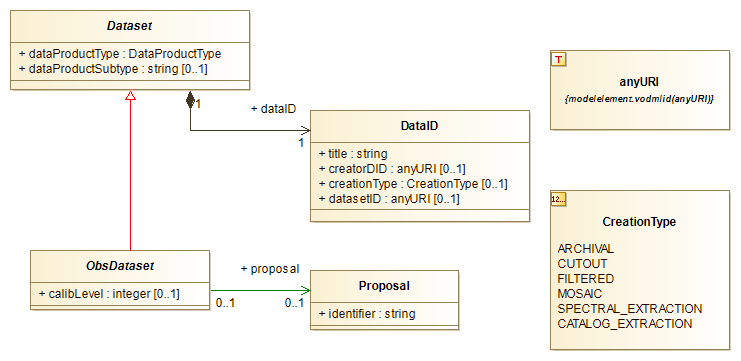
\includegraphics[width=0.9\textwidth]{diagrams/notation_example.png}}
    \caption{Notation example diagram}\label{fig:notation_example}
  \end{center}
  \end{figure}

  \subsection{ObjectType}
  \label{sect:ObjectType}
  ObjectTypes are represented by a plain box. The type name is annotated in the top window, abstract
types use italic typeface. Attributes, if any, are listed in the lower panel. Attributes may only be
of primitive type (real, string, etc), a defined DataType, or an Enumeration type. Relationships to
other objects are defined via the composition and reference relation arrows.

  \subsection{DataType}
  \label{sect:DataType}
  DataTypes are represented by a box shape similar to ObjectType, but annotated with a "T" symbol in the top left corner.

  \subsection{Enumerations}
  \label{sect:Enumerations}
  Enumerations are represented by a box shape similar to ObjectType, but annotated with a "1,2.."
symbol in the top left corner. Enumeration Literals (possible values) are listed below the
enumeration type name.

  \subsection{Generalization}
  \label{sect:Generalization}
  Generalizations are represented by a red line, with open triangle at the end of the source, or more general, object.

  \subsection{Composition}
  \label{sect:Composition}
  The composition relation is indicated by a black line with a solid diamond attached to the
containing object, and an arrow pointing to the object being contained. The composition relation is
very tight, where the container is responsible for the creation and existence of the target. Any
object may be in no more than one composition relation with any container. The attribute name
for the composition relation is annotated at the destination of the relation (e.g. "+ dataID"). This is
typically a lower-cased version of the destination type name, but this is not required.

  \subsection{Reference}
  \label{sect:Reference}
  The reference relation is indicated by a green line, with an arrow pointing to the object being
referenced. The reference relation is much looser than composition, the container has no
ownership of the target, but merely holds a pointer, or other indirect connection to it. The
attribute name is annotated at the destination of the relation ( e.g. "+ proposal"). This is typically
a lower-cased version of the destination type name, but may be another name indicating the role
that the element is playing in this context.

  \subsection{Multiplicity}
  \label{sect:Multiplicity}
  All attributes and relations have a multiplicity associated with them. For attributes, the multiplicity
is contained within brackets just after the attribute name. If no bracket is displayed, this is
equivalent to '[1]'.
\begin{itemize}
\item 1 = one and only one value must be provided.
\item 0..1 = zero or one value may be provided.
\item * = zero or more values may be provided (open ended).
\end{itemize}



% Appendix for IVOA Base types
\pagebreak
\section{Data Types}

  \subsection{Base Data Types}
  \label{sect:ivoa}
  Provides a set of standardized primitive data types as well as types for representing quantities
( values with associated units ). We provide a diagram of the model here, and refer the reader to
Section 5 of the VO-DML modeling specification document \citep{2018ivoa.spec.0910L} for more information.


    \begin{figure}[h]
    \begin{center}
      \fbox{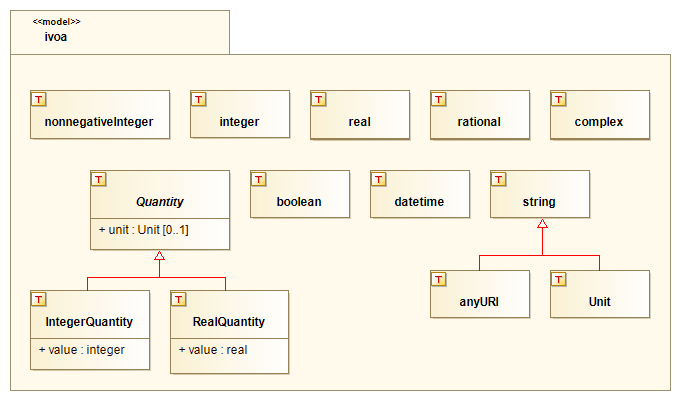
\includegraphics[width=0.9\textwidth]{diagrams/ivoa_types.png}}
      \caption{Base Data Types}\label{fig:basetypes}
    \end{center}
    \end{figure}

  \subsubsection{Units}
  \label{sect:Units}
  This model requires the use of the IVOA VOUnits Standard \citep{2014ivoa.spec.0523D} for representing units of physical
quantities. This standard reconciles common practices and current standards for use within the
IVOA community.

  \subsubsection{Dates}
  \label{sect:Dates}
  The 'datetime' datatype is for expressing date-time values. The string representation of a
datetime value should follow the FITS convention for representing dates. The FITS standard is
effectively ISO8601 format without the "Z" tag to indicate UTC (YYYY-MM-DDThh:mm:ss).
Values are nominally expressed in UTC.


\pagebreak
\bibliography{ivoatex/ivoabib,ivoatex/docrepo,other}


\end{document}
